\documentclass{beamer}

\usepackage[utf8]{inputenc}
\usepackage[T1]{fontenc}
\usepackage{lmodern}
\usepackage{amsmath,amssymb,amsfonts}
\usepackage{graphicx}
\usepackage[slovene]{babel}
\usepackage{tikz}
\usetikzlibrary{calc,3d}

% % Define the definition environment
\newtheorem{definition1}{Definicija}
\newtheorem{lemma1}{Lema}
\newtheorem{theorem1}{Izrek}

\title{Bernsteinovi polinomi treh spremenljivk}
\author{Petja Murnik in Nejc Jenko}
\date{\today}

\begin{document}

% Naslovni slide
\frame{\titlepage}

% Uvod
\section{Uvod}
\begin{frame}{Uvod}
    Pri predavanjih predmeta RPGO smo obravnavali Bernsteinove bazne polinome ene ter dveh spremenljivk, 
    ki smo jih uporabili pri različnih aplikacijah pri numerični matematiki.
    \newline
    V tem delu bomo predstavili Bernsteinove bazne polinome treh spremenljivk, ki so razširitev prej omenjenih.
\end{frame}

\section{Prostor $\mathcal{P}_d$}
\begin{frame}{Definicija prostora polinomov treh spremenljivk}
    Prostor polinomov stopnje $d$ treh spremenljivk je definiran kot:
    \[
      \mathcal{P}_d(x, y, z) = \left\{ \sum_{i+j+k \leq n} c_{i,j,k} x^i y^j z^k : c_{i,j,k} \in \mathbb{R} \right\}.
    \]
    Ta prostor ima dimenzijo:
    \[
        \mathcal{P}_d = \binom{d+3}{3}.
    \]
\end{frame}


\begin{frame}{Lema 1}
\begin{lemma1}
    Naj bo $\mathcal{P}_d$ definiran kot v prej.
    Potem velja, da je $\dim \mathcal{P}_d = \binom{d+3}{3} $. \\
    Nadalje monomi $\left\{x^i y^j z^k \right\}_{0 \le i  + j + k \le d}$ tvorijo njegovo bazo.
\end{lemma1}
\end{frame}


\begin{frame}{Dokaz leme 1 (skrajšan)}
    \begin{itemize}
        \item Monomi oblike $\{x^i y^j z^k\}_{0 \le i + j + k \le d}$ razpenjajo $\mathcal{P}_d$.
        \item Velja $|\{(i, j, k) : 0 \le i + j + k \le d, i, j, k \in \mathbb{N}_0\}| = \binom{d+3}{3} = \dim \mathcal{P}_d$.
        \item Predpostavimo, da je polinom $p(x, y, z) = \sum_{0 \le i + j + k \le d} a_{ijk} x^i y^j z^k$ identično enak 0.
        \item Vsi mešani odvodi polinoma so enaki 0.
        \item Direktno odvajanje: $D^i_x D^j_y D^k_z p(x, y, z)|_{x=0, y=0, z=0} = a_{ijk}$ za vsak $0 \le i + j + k \le d$.
        \item Linearna neodvisnost monomov je dokazana.
    \end{itemize}
\end{frame}


\begin{frame}{Lema 2}
\begin{lemma1}\label{lema_norma}
    Naj bo $T$ tetraeder z volumnom $V_T$, potem obstaja 
    konstanta $K$ odvisna le od $d$, da za vsak  $p \in \mathcal{P}_d$ ter $1 \le q < \infty$
    \begin{equation}
        V_T^{-1/q} \left\lVert p \right\rVert_{q,T} \le  \left\lVert p \right\rVert_{\infty l, T} \le K V_T^{-1/q} \left\lVert p \right\rVert_{q,T},
    \end{equation}
    kjer je $\left\lVert \dot{} \right\rVert_{q,T}$ standardna $L_q$ norma 
    glede na tetraeder $T$.
\end{lemma1}
\end{frame}


\begin{frame}{Dokaz leme 2}
    Za prvo neenakost računamo
    \begin{equation*}
        \int_{T} |p(t)|^q dt \le 
        \int_{T} \bigg( \sup_{t \in T} |p(t)| \bigg) ^q dt
        = \big(\sup_{t \in T} |p(t)| \big)^q \int_{T}1dt 
        = \left\lVert p \right\rVert_{\infty , T}^{q} V_T
    \end{equation*}
    ter če začetek in konec $q$-korenimo, dobimo željeno.
    
    Druga neenakost izhaja iz ekvivalentnosti norm v končno dimenzionalnem prostoru $\mathcal{P}_d$:
    \[
        \left\lVert p \right\rVert_{\infty, T} \leq K \left\lVert p \right\rVert_{q,T}.
    \]
    Združitev obeh neenakosti:
    \[
        V_T^{-1/q} \left\lVert p \right\rVert_{q,T} \leq K \left\lVert p \right\rVert_{\infty, T} \leq K V_T^{-1/q} \left\lVert p \right\rVert_{q,T}.
    \]
    S tem je lema dokazana.
\end{frame}

\section{Baricentrične koordinate glede na tetraeder}
\begin{frame}{Definicija nedegeneriranega tetraedra}
 \begin{definition1}
    Rečemo, da je tetraeder $T = \langle V_1, V_2, V_3, V_4 \rangle$ \textbf{nedegeneriran}, če ima neničelen volumen. Rečemo, da so vozlišča $V_1 , V_2 , V_3, V_4$ tetraedra $T$ v \textbf{kanoničnem redu}, če lahko $T$ rotiramo in transliramo  tako, da ploskev $\langle V_1, V_2, V_3\rangle$ leži v ravnini $z = 0$ in je pozitivno orientirana ter je $z$ koordinata vozlišča $V_4$ pozitivna.
\end{definition1}
\end{frame}



\begin{frame}{Lema 3}
\begin{lemma1}\label{lema_baricentricne}
    Naj bo $T = \langle V_1, V_2, V_3, V_4 \rangle$ tetraeder v kanoničnem redu.
    Potem za vsako točko $V = (x,y,z) \in \mathbb{R}^3$ obstajajo enolično določene
     $\phi_1, \phi_2, \phi_3, \phi_4 \in \mathbb{R}$,
    da velja 
    \begin{equation}\label{eq_baricentricne}
        V = \phi_1 V_1 + \phi_2 V_2 + \phi_3 V_3 + \phi_4 V_4
    \end{equation} ter 
    \begin{equation}\label{eq_particija}
        \phi_1 + \phi_2 + \phi_3 + \phi_4 = 1 .
    \end{equation}
    Vrednostim $\phi_1, \phi_2, \phi_3, \phi_4$ rečemo \textbf{baricentrične 
    koordinate} točke $V$ glede na tetraeder $T$.
\end{lemma1}
\end{frame}

\begin{frame}{Dokaz leme 3}
    Željeno je rešitev nesingularnega sistema
    \begin{align*}
        \begin{bmatrix}
            1 & 1 & 1 & 1 \\
            x_1 & x_2 & x_3 & x_4 \\
            y_1 & y_2 & y_3 & y_4 \\
            z_1 & z_2 & z_3 & z_4
        \end{bmatrix} 
        \begin{bmatrix}\phi_1 \\ \phi_2 \\ \phi_3 \\ \phi_4 \end{bmatrix} = \begin{bmatrix}
            1 \\ x \\ y \\ z \end{bmatrix}.
        \qed
    \end{align*}

    \begin{align*}\label{eq_cramer}
        \phi_1 = \frac{1}{\text{det}(M)}
        \begin{vmatrix}
            1 & 1 & 1 & 1 \\
            x & x_2 & x_3 & x_4 \\
            y & y_2 & y_3 & y_4 \\
            z & z_2 & z_3 & z_4
        \end{vmatrix}
        = \frac{V_{\widetilde{T_1}}}{V_T},
    \end{align*}
    kjer je $V_{\widetilde{T_i}}$
    prostornina tetraedra, ki ga dobimo, če zamenjamo $i$-to vozlišče
    s točko $V$.
\end{frame}

\begin{frame}{Baricentrične koordinate glede na tetraeder}
    \centering
    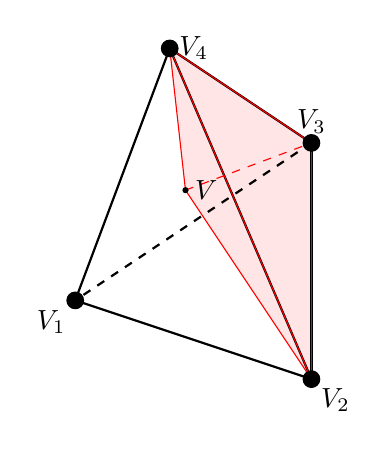
\begin{tikzpicture}[scale=3, z={(0.4cm,0.4cm)}] 
        % Define vertices of the tetrahedron
        \coordinate (V_1) at (0, 1/3, 0);
        \coordinate (V_2) at (1, 0, 0);
        \coordinate (V_3) at (1,1,0);
        \coordinate (V_4) at (0,1,1);
        \coordinate (V) at (1/3,2/3,1/3);




        % Fill faces with light red
        \fill[red!10] (V) -- (V_2) -- (V_3) -- cycle;
        \fill[red!10] (V) -- (V_2) -- (V_4) -- cycle;
        \fill[red!10] (V) -- (V_3) -- (V_4) -- cycle;
        \fill[red!10] (V_2) -- (V_3) -- (V_4) -- cycle;
        

        % Draw edges
        \draw[thick] (V_1) -- (V_2);
        \draw[thick] (V_2) -- (V_3);
        \draw[thick] (V_1) -- (V_4);
        \draw[thick] (V_2) -- (V_4);
        \draw[thick] (V_3) -- (V_4);
        \draw[thick, dashed] (V_3) -- (V_1);



        \draw[red] (V) -- (V_4);
        \draw[red] (V) -- (V_2);
        \draw[red, dashed] (V) -- (V_3);
        \draw[red] (V_2) -- (V_3);
        \draw[red] (V_4) -- (V_3);
        \draw[red] (V_2) -- (V_4);


        % Add vertices
        \filldraw[black] (V_1) circle (1pt) node[below left] {$V_1$};
        \filldraw[black] (V_2) circle (1pt) node[below right] {$V_2$};
        \filldraw[black] (V_3) circle (1pt) node[above] {$V_3$};
        \filldraw[black] (V_4) circle (1pt) node[right] {$V_4$};
        \filldraw[black] (V) circle (0.3pt) node[right] {$V$};


    \end{tikzpicture}
\end{frame}


% Definicija Bernsteinovih baznih polinomov
\section{Bernsteinovi bazni polinomi}
\begin{frame}{Definicija Bernsteinovih baznih polinomov}
\begin{definition1}
    Naj bo $T = \langle V_1, V_2, V_3, V_4 \rangle$ tetraeder v kanoničnem redu.
    \textbf{Bernsteinov bazni polinom} stopnje $n$ glede na tetraeder $T$ je definiran kot
    \begin{equation}
        B_{ijkl}^d := \frac{d!}{i!j!k!l!} \phi_1^i \phi_2^j \phi_3^k \phi_4^l, \quad i + j + k + l = d,
    \end{equation}
    kjer je $\phi_1, \phi_2, \phi_3, \phi_4$ baricentrične koordinate funkcije
    glede na tetraeder $T$. V primeru, ko je kateri izmed indeksov $i, j, k, l$ negativen, 
    nastavimo $B_{ijkl}^d = 0$.
\end{definition1}
    Ključne lastnosti: nenegativnost, particija enote.
\end{frame}

\begin{frame}{Izrek 2}
\begin{theorem1}\label{izrek_bernstein}
    Bernsteinovi bazni polinomi $B_{ijkl}^d$ tvorijo bazo prostora $\mathcal{P}_d$.
    Prav tako velja 
    \begin{equation}\label{eq_partcija_enote}
        \sum_{i+j+k+l = d} B_{ijkl}^d(V) = 1, \quad \forall V \in \mathbb{R}^3     
    \end{equation}
    ter
    \begin{equation}
        0 \leq B_{ijkl}^d(V) \leq 1, \quad \forall V \in T.
    \end{equation}
\end{theorem1}
\end{frame}

\begin{frame}{Povzetek dokaza}
    \begin{itemize}
        \item Označimo z $\mathcal{B}_d$ množico Bernsteinovih polinomov.
        \item Dokazujemo enakost $\left( \phi_1 + \phi_2 + \phi_3 + \phi_4 \right)^d = \sum_{i+j+k+l = d} \frac{d!}{i!j!k!l!} \phi_1^i \phi_2^j \phi_3^k \phi_4^l$.
        \item Indukcija po $d$:
        \begin{itemize}
            \item Za $d = 0$ je enakost očitna.
            \item Za $d = 1$ uporabimo enačbo baricentričnih koordinat.
            \item Združimo vse člene in dobimo $\sum_{i+j+k+l = d} \frac{ix_1 + jx_2 + k x_3 + l x_4}{d} B_{ijkl}^d$.
        \end{itemize}
        \item Indukcijski korak:
        \begin{itemize}
            \item Predpostavimo, da trditev velja za $\mu + \nu + \kappa \leq d-1$.
            \item Za $\mu + \nu + \kappa = d$ uporabimo podobno metodo kot za $d = 1$.
        \end{itemize}
        \item Dokazujemo, da Bernsteinovi bazni polinomi tvorijo bazo $\mathcal{P}_d$.
        \item Iz lastnosti baricentričnih koordinat sledi izjava o mejah Bernsteinovih baznih funkcij.
    \end{itemize}
\end{frame}

\begin{frame}{Povzetek dokaza}
    \begin{itemize}
        \item Dokazali smo, da Bernsteinovi polinomi tvorijo bazo prostora $\mathcal{P}_d$.
        \item Uporabili smo indukcijo po $d$ in lastnosti baricentričnih koordinat.
        \item Izjava o mejah Bernsteinovih baznih funkcij sledi direktno iz teh lastnosti.
    \end{itemize}
\end{frame}

\section{B-forma in B-koeficienti}
\begin{frame}{Definicija B-forme in B-koeficientov}
Iz izreka \ref{izrek_bernstein} sledi, da lahko vsak polinom $p \in \mathcal{P}_d$
lahko zapišemo na enoličen način kot
\begin{equation}\label{eq_Bforma}
    p = \sum_{i+j+k+l = d} c_{ijkl} B_{ijkl}^d.
\end{equation}
Tak zapis imenujemo \textbf{B-forma} ter koeficente $c_{ijkl}$ \textbf{B-koeficienti}.
Množico domenskih točk definiramo ter označimo kot
\begin{equation}
    \mathcal{D}_{d,T} := 
    \left\{
        \zeta_{ijkl}^T:= \frac{i V_1 + j V_2 + k V_3 + l V_4}{d}
     \right\}_{i + j+ k+l = d}.
\end{equation}
\end{frame}

\begin{frame}{Domenske točke $\mathcal{D}_{3,T}$}
    \centering
    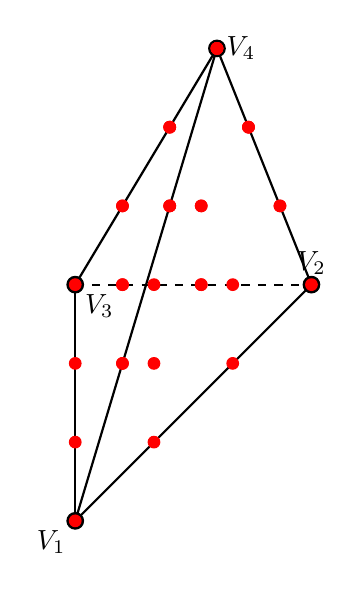
\begin{tikzpicture}[scale=3, z={(0.6cm,2cm)}] 
        % Define vertices of the tetrahedron
        \coordinate (V_1) at (0, 0, 0);
        \coordinate (V_2) at (0,1, 0);
        \coordinate (V_3) at (1,1,0);
        \coordinate (V_4) at (0,0,1);

        % Draw edges
        \draw[thick] (V_1) -- (V_2);
        \draw[thick,dashed] (V_2) -- (V_3);
        \draw[thick] (V_1) -- (V_4);
        \draw[thick] (V_2) -- (V_4);
        \draw[thick] (V_3) -- (V_4);
        \draw[thick] (V_3) -- (V_1);

        % Add vertice
        \filldraw[black] (V_1) circle (1pt) node[below left] {$V_1$};
        \filldraw[black] (V_2) circle (1pt) node[below right] {$V_3$};
        \filldraw[black] (V_3) circle (1pt) node[above] {$V_2$};
        \filldraw[black] (V_4) circle (1pt) node[right] {$V_4$};


        \coordinate (V_0_0_3) at (0.0, 0.0, 1.0);
        \filldraw[red,] (V_0_0_3) circle (0.7pt);
        \coordinate (V_0_0_3) at (0.0, 0.0, 1.0);
        \filldraw[red,] (V_0_0_3) circle (0.7pt);
        \coordinate (V_0_0_3) at (0.0, 0.0, 1.0);
        \filldraw[red,] (V_0_0_3) circle (0.7pt);
        \coordinate (V_0_0_3) at (0.0, 0.0, 1.0);
        \filldraw[red,] (V_0_0_3) circle (0.7pt);
        \coordinate (V_0_0_2) at (0.3333333333333333, 0.3333333333333333, 0.6666666666666666);
        \filldraw[red,] (V_0_0_2) circle (0.7pt);
        \coordinate (V_0_0_2) at (0.3333333333333333, 0.3333333333333333, 0.6666666666666666);
        \filldraw[red,] (V_0_0_2) circle (0.7pt);
        \coordinate (V_0_0_2) at (0.3333333333333333, 0.3333333333333333, 0.6666666666666666);
        \filldraw[red,] (V_0_0_2) circle (0.7pt);
        \coordinate (V_0_0_1) at (0.6666666666666666, 0.6666666666666666, 0.3333333333333333);
        \filldraw[red,] (V_0_0_1) circle (0.7pt);
        \coordinate (V_0_0_1) at (0.6666666666666666, 0.6666666666666666, 0.3333333333333333);
        \filldraw[red,] (V_0_0_1) circle (0.7pt);
        \coordinate (V_0_0_0) at (1.0, 1.0, 0.0);
        \filldraw[red,] (V_0_0_0) circle (0.7pt);
        \coordinate (V_0_1_2) at (0.0, 0.3333333333333333, 0.6666666666666666);
        \filldraw[red,] (V_0_1_2) circle (0.7pt);
        \coordinate (V_0_1_2) at (0.0, 0.3333333333333333, 0.6666666666666666);
        \filldraw[red,] (V_0_1_2) circle (0.7pt);
        \coordinate (V_0_1_2) at (0.0, 0.3333333333333333, 0.6666666666666666);
        \filldraw[red,] (V_0_1_2) circle (0.7pt);
        \coordinate (V_0_1_1) at (0.3333333333333333, 0.6666666666666666, 0.3333333333333333);
        \filldraw[red,] (V_0_1_1) circle (0.7pt);
        \coordinate (V_0_1_1) at (0.3333333333333333, 0.6666666666666666, 0.3333333333333333);
        \filldraw[red,] (V_0_1_1) circle (0.7pt);
        \coordinate (V_0_1_0) at (0.6666666666666666, 1.0, 0.0);
        \filldraw[red,] (V_0_1_0) circle (0.7pt);
        \coordinate (V_0_2_1) at (0.0, 0.6666666666666666, 0.3333333333333333);
        \filldraw[red,] (V_0_2_1) circle (0.7pt);
        \coordinate (V_0_2_1) at (0.0, 0.6666666666666666, 0.3333333333333333);
        \filldraw[red,] (V_0_2_1) circle (0.7pt);
        \coordinate (V_0_2_0) at (0.3333333333333333, 1.0, 0.0);
        \filldraw[red,] (V_0_2_0) circle (0.7pt);
        \coordinate (V_0_3_0) at (0.0, 1.0, 0.0);
        \filldraw[red,] (V_0_3_0) circle (0.7pt);
        \coordinate (V_1_0_2) at (0.0, 0.0, 0.6666666666666666);
        \filldraw[red,] (V_1_0_2) circle (0.7pt);
        \coordinate (V_1_0_2) at (0.0, 0.0, 0.6666666666666666);
        \filldraw[red,] (V_1_0_2) circle (0.7pt);
        \coordinate (V_1_0_2) at (0.0, 0.0, 0.6666666666666666);
        \filldraw[red,] (V_1_0_2) circle (0.7pt);
        \coordinate (V_1_0_1) at (0.3333333333333333, 0.3333333333333333, 0.3333333333333333);
        \filldraw[red,] (V_1_0_1) circle (0.7pt);
        \coordinate (V_1_0_1) at (0.3333333333333333, 0.3333333333333333, 0.3333333333333333);
        \filldraw[red,] (V_1_0_1) circle (0.7pt);
        \coordinate (V_1_0_0) at (0.6666666666666666, 0.6666666666666666, 0.0);
        \filldraw[red,] (V_1_0_0) circle (0.7pt);
        \coordinate (V_1_1_1) at (0.0, 0.3333333333333333, 0.3333333333333333);
        \filldraw[red,] (V_1_1_1) circle (0.7pt);
        \coordinate (V_1_1_1) at (0.0, 0.3333333333333333, 0.3333333333333333);
        \filldraw[red,] (V_1_1_1) circle (0.7pt);
        \coordinate (V_1_1_0) at (0.3333333333333333, 0.6666666666666666, 0.0);
        \filldraw[red,] (V_1_1_0) circle (0.7pt);
        \coordinate (V_1_2_0) at (0.0, 0.6666666666666666, 0.0);
        \filldraw[red,] (V_1_2_0) circle (0.7pt);
        \coordinate (V_2_0_1) at (0.0, 0.0, 0.3333333333333333);
        \filldraw[red,] (V_2_0_1) circle (0.7pt);
        \coordinate (V_2_0_1) at (0.0, 0.0, 0.3333333333333333);
        \filldraw[red,] (V_2_0_1) circle (0.7pt);
        \coordinate (V_2_0_0) at (0.3333333333333333, 0.3333333333333333, 0.0);
        \filldraw[red,] (V_2_0_0) circle (0.7pt);
        \coordinate (V_2_1_0) at (0.0, 0.3333333333333333, 0.0);
        \filldraw[red,] (V_2_1_0) circle (0.7pt);
        \coordinate (V_3_0_0) at (0.0, 0.0, 0.0);
        \filldraw[red,] (V_3_0_0) circle (0.7pt);

        % \coordinate (V_0_0_2) at (0.0, 0.0, 1.0);
        % \filldraw[red,] (V_0_0_2) circle (0.7pt);
        % \coordinate (V_0_0_2) at (0.0, 0.0, 1.0);
        % \filldraw[red,] (V_0_0_2) circle (0.7pt);
        % \coordinate (V_0_0_2) at (0.0, 0.0, 1.0);
        % \filldraw[red,] (V_0_0_2) circle (0.7pt);
        % \coordinate (V_0_0_1) at (0.5, 0.5, 0.5);
        % \filldraw[red,] (V_0_0_1) circle (0.7pt);
        % \coordinate (V_0_0_1) at (0.5, 0.5, 0.5);
        % \filldraw[red,] (V_0_0_1) circle (0.7pt);
        % \coordinate (V_0_0_0) at (1.0, 1.0, 0.0);
        % \filldraw[red,] (V_0_0_0) circle (0.7pt);
        % \coordinate (V_0_1_1) at (0.0, 0.5, 0.5);
        % \filldraw[red,] (V_0_1_1) circle (0.7pt);
        % \coordinate (V_0_1_1) at (0.0, 0.5, 0.5);
        % \filldraw[red,] (V_0_1_1) circle (0.7pt);
        % \coordinate (V_0_1_0) at (0.5, 1.0, 0.0);
        % \filldraw[red,] (V_0_1_0) circle (0.7pt);
        % \coordinate (V_0_2_0) at (0.0, 1.0, 0.0);
        % \filldraw[red,] (V_0_2_0) circle (0.7pt);
        % \coordinate (V_1_0_1) at (0.0, 0.0, 0.5);
        % \filldraw[red,] (V_1_0_1) circle (0.7pt);
        % \coordinate (V_1_0_1) at (0.0, 0.0, 0.5);
        % \filldraw[red,] (V_1_0_1) circle (0.7pt);
        % \coordinate (V_1_0_0) at (0.5, 0.5, 0.0);
        % \filldraw[red,] (V_1_0_0) circle (0.7pt);
        % \coordinate (V_1_1_0) at (0.0, 0.5, 0.0);
        % \filldraw[red,] (V_1_1_0) circle (0.7pt);
        % \coordinate (V_2_0_0) at (0.0, 0.0, 0.0);
        % \filldraw[red,] (V_2_0_0) circle (0.7pt);
    \end{tikzpicture}
    $V_1 = (0, 0, 0), V_2 =(0,1, 0), V_3 = (1,1,0), V_4 = (0,0,1) $
\end{frame}


\begin{frame}{Izrek 3}
\begin{theorem1}
    Naj bo $p \in \mathcal{P}_d$ zapisan v obliki \eqref{eq_Bforma}. Označimo 
    z $\text{F}_1 := \langle V_2,V_3,V_4 \rangle$ ploskev tetraedra $T$ nasproti vozlišču $V_1$.
    Potem velja 
    \begin{equation}
        p|_{\text{F}_1} = \sum_{j+k+l = d} c_{0jkl}B_{0jkl}^d = 
            \sum_{j+k+l}c_{jkl}^{\text{F}_1} B_{jkl}^{\text{F}_1,d},
    \end{equation}
    kjer $c_{jkl}^{\text{F}_1}:=c_{0jkl}$ ter so $B_{jkl}^{\text{F}_1,d}$
    Bernsteinovi bazni polinomi stopnje $d$ glede na trikotnik $\text{F}_1$ .
\end{theorem1}
\end{frame}

% De Casteljaujev algoritem
\section{De Casteljaujev algoritem}
\begin{frame}{Ideja De Casteljaujevega algoritma}
V tem razdelku bomo predstavili de Casteljaujev algoritem. Algoritem omogoča učinkovito in stabilno izračunavanje vrednosti polinomov v B-formi. Algoritem temelji na rekurzivni zvezi:

\begin{align*}
 B_{ijkl}^d = \phi_1 B_{i-1,j,k,l}^{d-1} + \phi_2 B_{i,j-1,k,l}^{d-1} + \phi_3 B_{i,j,k-1,l}^{d-1} + \phi_4 B_{i,j,k,l-1}^{d-1}, 
\end{align*}
\end{frame}


\begin{frame}{Izrek 4}
\begin{theorem1}
    Naj bo $p \in \mathcal{P}_d$ zapisan v obliki B-forme \eqref{eq_Bforma}. Njegove koeficiente označimo z $c_{ijkl}^{(0)} = c_{ijkl}, i+j+l+k = d$.
    Naj ima točka $V$ baricentrične koordinate $\phi_1, \phi_2, \phi_3, \phi_4$.

    Potem velja:
    $$
    p(V) = \sum_{i+j+k+l = d} c_{ijkl}^{(d)} B_{ijkl}^d(V),
    $$

    kjer so  $c_{ijkl}^{(r)}$ definirani kot:
    \begin{align*}
        c_{ijkl}^{(r)} = \phi_1 c_{i-1,j,k,l}^{(r-1)} + \phi_2 c_{i,j-1,k,l}^{(r-1)} + \phi_3 c_{i,j,k-1,l}^{(r-1)} + \phi_4 c_{i,j,k,l-1}^{(r-1)},
    \end{align*}
    za i+j+k+l = d, r = 1, 2, \ldots, d.
\end{theorem1}
\end{frame}


\begin{frame}{Algoritem 1}
de Casteljaujev algoritem
    \begin{enumerate}
        \item Za $r = 0$ nastavi $c_{ijkl}^{(0)} = c_{ijkl}$ za $i+j+k+l = d$.
        \item Za $r = 1, 2, \ldots, d$ izračunaj
        \begin{align*}
            c_{ijkl}^{(r)} = \phi_1 c_{i-1,j,k,l}^{(r-1)} + \phi_2 c_{i,j-1,k,l}^{(r-1)} + \phi_3 c_{i,j,k-1,l}^{(r-1)} + \phi_4 c_{i,j,k,l-1}^{(r-1)},
        \end{align*}
        za $i+j+k+l = d$.
        \item Vrednost polinoma $p$ v točki $V$ je enaka
        \begin{align*}
            p(V) = \sum_{i+j+k+l = d} c_{ijkl}^{(d)} B_{ijkl}^d(V).
        \end{align*}
    \end{enumerate}

\end{frame}

\end{document}
